\documentclass{article}

\usepackage[final]{neurips_2026}
\usepackage[utf8]{inputenc}
\usepackage[T1]{fontenc}
\usepackage[hidelinks]{hyperref}
\usepackage{url}
\usepackage{booktabs}
\usepackage{amsfonts}
\usepackage{amsmath}
\usepackage{microtype}
\usepackage{graphicx}
\usepackage{subcaption}
\usepackage{xcolor}
\usepackage{pifont}
\usepackage{enumitem}
\usepackage{tabularx}
\usepackage{array}
\newcolumntype{Y}{>{\raggedright\arraybackslash}X}
\setlist{nosep,leftmargin=*}

\newcommand{\cmark}{\ding{51}}
\newcommand{\grade}[1]{\textbf{\textcolor{blue!70!black}{[#1]}}}

\graphicspath{{figures/}}

\title{Scaling Laws and Accuracy--Efficiency Trade-offs in Modern ConvNets on CIFAR-10}

\author{%
  Boyi Shi \qquad Puhao Zhu \qquad Jinye Gong \\
  Group 148 --- DD2424 Deep Learning in Data Science, KTH \\
}

\begin{document}
\maketitle

\begin{abstract}
  On CIFAR-10 ($32{\times}32$), we ask whether ConvNeXt-style blocks improve the accuracy--FLOPs trade-off versus a strong VGG baseline when compute is matched.
  We implement a unified PyTorch stack (fixed 45k/5k train/val split, AdamW, cosine annealing with warmup, 200 epochs, seed 42) and train \textbf{17/17} planned runs: three block families (VGG, depthwise separable, ConvNeXt) at low ($\sim$150M), medium ($\sim$310M), and high ($\sim$460M) FLOPs tiers, plus width, kernel ($k{\in}\{3,5,7,11\}$), and depth ablations.
  \textbf{Key results:} best model \texttt{vgg\_baseline} $w{=}64$---309.5M FLOPs, \textbf{92.78\%} test; VGG wins every matched tier; depthwise reaches 92.18\% at $\sim$90\% of VGG FLOPs (99.4\% of VGG accuracy); ConvNeXt never beats VGG/DW at matched budgets; kernel size increases monotonically \emph{hurt} both modern families ($\sim$3.7 pt drop at $k{=}11$ vs.\ $k{=}3$).
  We report Pareto fronts, marginal gains per FLOP, and budget-aware design rules mapped to Default Project grades \grade{E}, \grade{D/C}, and \grade{B/A}.
\end{abstract}

\section{Introduction}

CIFAR-10 is a standard 10-class, $32{\times}32$ benchmark. ConvNets evolved from VGG-style $3{\times}3$ stacks to depthwise separable convolutions (MobileNet) and ConvNeXt blocks with large depthwise kernels, LayerNorm, and inverted bottlenecks~\cite{liu2022convnext}. Many modern designs target ImageNet resolution; on low-resolution inputs it is unclear whether large receptive fields still help.

\textbf{Misleading default comparison.} At $w{=}64$, our templates use 309.5M FLOPs (VGG), 40.4M (depthwise), and 462.4M (ConvNeXt)---13\% and 149\% of VGG compute respectively (Table~\ref{tab:baseline}). Raw test accuracy therefore cannot answer RQ1. We must align FLOPs budgets and scan width, kernel, and depth.

\textbf{Research questions (Group 148 proposal).}
\textbf{RQ1:} Do ConvNeXt-style blocks provide a better accuracy--FLOPs trade-off than a strong VGG baseline on CIFAR-10?
\textbf{RQ2:} How do depth, width, kernel size, and block type scale with budget, and which direction gives the largest marginal test gain per extra FLOP?

\textbf{Contributions.} (i) Reproducible training/evaluation with fixed val indices and \texttt{thop} FLOPs ($=2\times$MACs); (ii) strong VGG baseline at 92.78\% test; (iii) nine FLOPs-matched tier runs (3$\times$3 block types); (iv) kernel scan (7/7) and depth variants (2/2); (v) Pareto analysis and design rules.

We follow DD2424 Default Project~2~\cite{dd2424default2026}; Table~\ref{tab:grades} maps course grades to our deliverables (target A/B).

\begin{table}[t]
  \caption{Default Project~2 grades vs.\ Group~148 deliverables.}
  \label{tab:grades}
  \centering
  \footnotesize
  \begin{tabularx}{\linewidth}{@{}c c Y Y@{}}
    \toprule
    \textbf{Grade} & & \textbf{Course requirement} & \textbf{Our deliverable} \\
    \midrule
    \grade{E} & \cmark &
      PyTorch VGG; AdamW; dropout, weight decay, augmentation, BN; schedulers; high test accuracy &
      \S\ref{sec:e}: \textbf{92.78\%} test \\
    \grade{D/C} & \cmark &
      $\geq$2 extension directions (modern recipe, architectural scaling, etc.) &
      (1)~warmup+cosine; (2)~width scaling; LayerNorm in ConvNeXt \\
    \grade{B/A} & \cmark &
      Fair modern vs.\ VGG comparison; ablations; clear RQs &
      17 runs; Pareto analysis; design rules (\S\ref{sec:conc}) \\
    \bottomrule
  \end{tabularx}
\end{table}

\section{Method and experimental protocol}

\subsection{Dataset and reproducible pipeline}

CIFAR-10: 50k train / 10k test, 10 classes. We hold out 5k val ($\texttt{val\_ratio}{=}0.1$, $\texttt{seed}{=}42$); indices saved in \texttt{cifar10\_val\_indices.pt}. Test is evaluated \emph{once} per run after training; all model selection uses val only.

\subsection{Training recipe (\grade{E}+\grade{D/C})}

Table~\ref{tab:hyper}. Implementation: \texttt{train/pipeline.py}, \texttt{train/trainer.py}. MixUp and AMP are \textbf{disabled} for all ablations (team protocol).

\begin{table}[t]
  \caption{Unified hyperparameters (\texttt{configs/default.yaml}).}
  \label{tab:hyper}
  \centering
  \footnotesize
  \begin{tabular}{@{}ll@{}}
    \toprule
    Key & Value \\
    \midrule
    seed / val\_ratio & 42 / 0.1 \\
    batch\_size / epochs & 128 / 200 \\
    optimizer & AdamW~\cite{loshchilov2019adamw}, lr $10^{-3}$, wd 0.05 \\
    scheduler & cosine + 5-epoch warmup, $\mathrm{min\_lr}{=}10^{-6}$ \\
    augmentation & RandomCrop(32, pad=4), horizontal flip \\
    regularization & dropout 0.5; BN in VGG/DW \\
    \bottomrule
  \end{tabular}
\end{table}

\subsection{Model families (\grade{E}+\grade{B/A})}

\textbf{VGG} (\texttt{vgg\_baseline}): Conv--BN--ReLU, three max-pools, MLP head; \texttt{width} tunable.
\textbf{Depthwise} (\texttt{depthwise\_small}): DW $k{\times}k$ + PW $1{\times}1$, BN, ReLU; same stage layout as VGG; \texttt{width}, \texttt{kernel\_size}.
\textbf{ConvNeXt} (\texttt{convnext\_small}): stem, ConvNeXt blocks (large-kernel DW, LayerNorm2d, inverted bottleneck, residual), GAP + linear head; \texttt{width}, \texttt{depths}, \texttt{kernel\_size}.

\begin{table}[t]
  \caption{Default structure at $\texttt{width}{=}64$.}
  \label{tab:struct}
  \centering
  \footnotesize
  \begin{tabular}{@{}lcccc@{}}
    \toprule
    Model & width & kernel & depths & dropout \\
    \midrule
    VGG & 64 & 3 & --- & 0.5 \\
    Depthwise & 64 & 3 & --- & 0.5 \\
    ConvNeXt & 64 & 7 & (2,2,2) & 0.5 \\
    \bottomrule
  \end{tabular}
\end{table}

\subsection{FLOPs matching and experiment phases}

FLOPs: \texttt{thop} on $[1,3,32,32]$; report FLOPs $= 2\times$MACs. Tiers: low $\sim$150M, med $\sim$310M, high $\sim$460M ($\pm10\%$), aligned by sweeping \texttt{width} (\texttt{configs/experiments.yaml}).

\textbf{Execution (2026-05).} Phase~1 [\grade{E}]: train \texttt{vgg\_baseline} $w{=}64$. Phase~2 [\grade{B/A}]: nine tier-aligned runs. Phase~3: kernel scan at CN $w{=}52$, DW $w{=}175$. Phase~4: CN depth shallow $(1,1,1)$ and deep $(3,3,3)$---shallow run retrained after a 2-epoch interruption (41.67\% test). All jobs via \texttt{scripts/run\_experiments.py}; metrics in \texttt{logs/results.csv}.

\begin{table}[t]
  \caption{Experiment queue (17/17 completed, 200 epochs each).}
  \label{tab:queue}
  \centering
  \scriptsize
  \setlength{\tabcolsep}{1.5pt}
  \begin{tabular}{@{}lllr@{}}
    \toprule
    Phase & Config & FLOPs & Test \\
    \midrule
    \grade{E} & VGG $w{=}64$ & 309.5M & 92.78\% \\
    \grade{B/A} low & VGG/DW/CN 48/128/32 & 175/152/122M & 92.05/90.86/88.85\% \\
    \grade{B/A} med & VGG/DW/CN 64/175/52 & 310/280/309M & 92.78/92.18/90.34\% \\
    \grade{B/A} high & VGG/DW/CN 80/224/64 & 482/453/462M & 92.46/92.15/90.12\% \\
    kernel & CN $w{=}52$, $k{=}3,5,7,11$ & 294--336M & 91.85--88.21\% \\
    kernel & DW $w{=}175$, $k{=}3,5,7,11$ & 280--366M & 92.18--88.49\% \\
    depth & CN $(1,1,1)$ / $(3,3,3)$ & 250/313M & 89.16/90.27\% \\
    \bottomrule
  \end{tabular}
\end{table}

\section{Results}
\label{sec:results}

\subsection{Summary of findings}

\begin{table}[t]
  \caption{Core findings (test accuracy unless noted).}
  \label{tab:findings}
  \centering
  \footnotesize
  \begin{tabularx}{\linewidth}{@{}c l Y@{}}
    \toprule
    \# & Finding & Evidence \\
    \midrule
    F1 & Global best: VGG $w{=}64$, 92.78\% @ 309.5M & Tables~\ref{tab:baseline}, \ref{tab:pareto} \\
    F2 & VGG highest test in all three FLOPs tiers & Table~\ref{tab:tier} \\
    F3 & DW med: 92.18\% @ 90\% VGG FLOPs (99.4\% of VGG acc.) & Table~\ref{tab:tier} \\
    F4 & CN lowest every tier; high tier 90.12\% $<$ med-tier VGG & Table~\ref{tab:tier} \\
    F5 & VGG $w{=}80$ worse than $w{=}64$ despite +172M FLOPs & Tables~\ref{tab:tier}, \ref{tab:marginal} \\
    F6--F7 & Kernel $\uparrow$ $\Rightarrow$ test $\downarrow$; $k{=}11$ worst & Table~\ref{tab:kernel} \\
    F8 & CN depth: $(3,3,3)$ $>$ $(1,1,1)$; both $\ll$ VGG/DW & Table~\ref{tab:depth} \\
    F9 & Unaligned defaults cannot answer RQ1 & Table~\ref{tab:baseline} \\
    \bottomrule
  \end{tabularx}
\end{table}

\subsection{\grade{E} VGG baseline}
\label{sec:e}

Table~\ref{tab:baseline}: at $w{=}64$, VGG reaches val \textbf{93.92\%}, test \textbf{92.78\%} (checkpoint near epoch 197). Fig.~\ref{fig:vgg}: val saturates after $\sim$100 epochs; train $\rightarrow$100\% indicates mild overfitting, yet test exceeds the E-level ``high eighties'' target.

\begin{table}[t]
  \caption{Unaligned $w{=}64$ profiles (200 epochs).}
  \label{tab:baseline}
  \centering
  \footnotesize
  \begin{tabular}{@{}lrrrr@{}}
    \toprule
    Model & Params & FLOPs & Val & Test \\
    \midrule
    VGG & 2,197,706 & 309.5M & \textbf{93.92\%} & \textbf{92.78\%} \\
    ConvNeXt & 1,662,666 & 462.4M & 91.40\% & 90.12\% \\
    Depthwise & 1,186,149 & 40.4M & 91.20\% & 89.58\% \\
    \bottomrule
  \end{tabular}
\end{table}

\begin{figure}[t]
  \centering
  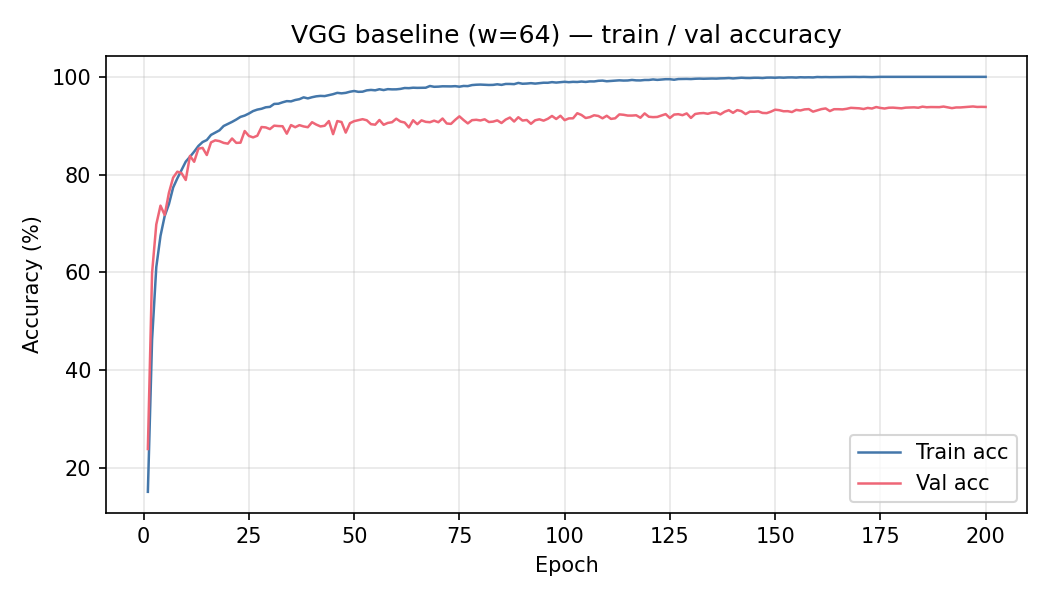
\includegraphics[width=0.58\linewidth]{vgg_baseline_train_val.png}
  \caption{\grade{E} VGG train/val curves ($w{=}64$).}
  \label{fig:vgg}
\end{figure}

\subsection{\grade{B/A} FLOPs-matched block comparison}
\label{sec:ba}

Table~\ref{tab:tier} (core RQ1). \textbf{Analysis:} (1) VGG wins all tiers. (2) Med DW: 92.18\% at 279.6M FLOPs vs.\ VGG 92.78\% at 309.5M---best efficiency. (3) CN trails by 1.2--3.2 pt per tier; at high budget (462M) still below med VGG. (4) VGG $w{=}80$ underperforms $w{=}64$ (possible overfitting).

\begin{table}[t]
  \caption{FLOPs-matched tiers (val / test \%).}
  \label{tab:tier}
  \centering
  \footnotesize
  \begin{tabular}{@{}llrrr@{}}
    \toprule
    Tier & Model (width) & FLOPs & Val & Test \\
    \midrule
    Low & VGG (48) & 175.1M & 92.58 & \textbf{92.05} \\
    Low & DW (128) & 152.1M & 92.42 & 90.86 \\
    Low & CN (32) & 122.1M & 89.80 & 88.85 \\
    Med & VGG (64) & 309.5M & 93.92 & \textbf{92.78} \\
    Med & DW (175) & 279.6M & 92.46 & 92.18 \\
    Med & CN (52) & 309.2M & 90.70 & 90.34 \\
    High & VGG (80) & 481.9M & 93.40 & \textbf{92.46} \\
    High & DW (224) & 453.4M & 92.88 & 92.15 \\
    High & CN (64) & 462.4M & 91.40 & 90.12 \\
    \bottomrule
  \end{tabular}
\end{table}

\begin{figure}[t]
  \centering
  \begin{subfigure}[t]{0.48\linewidth}
    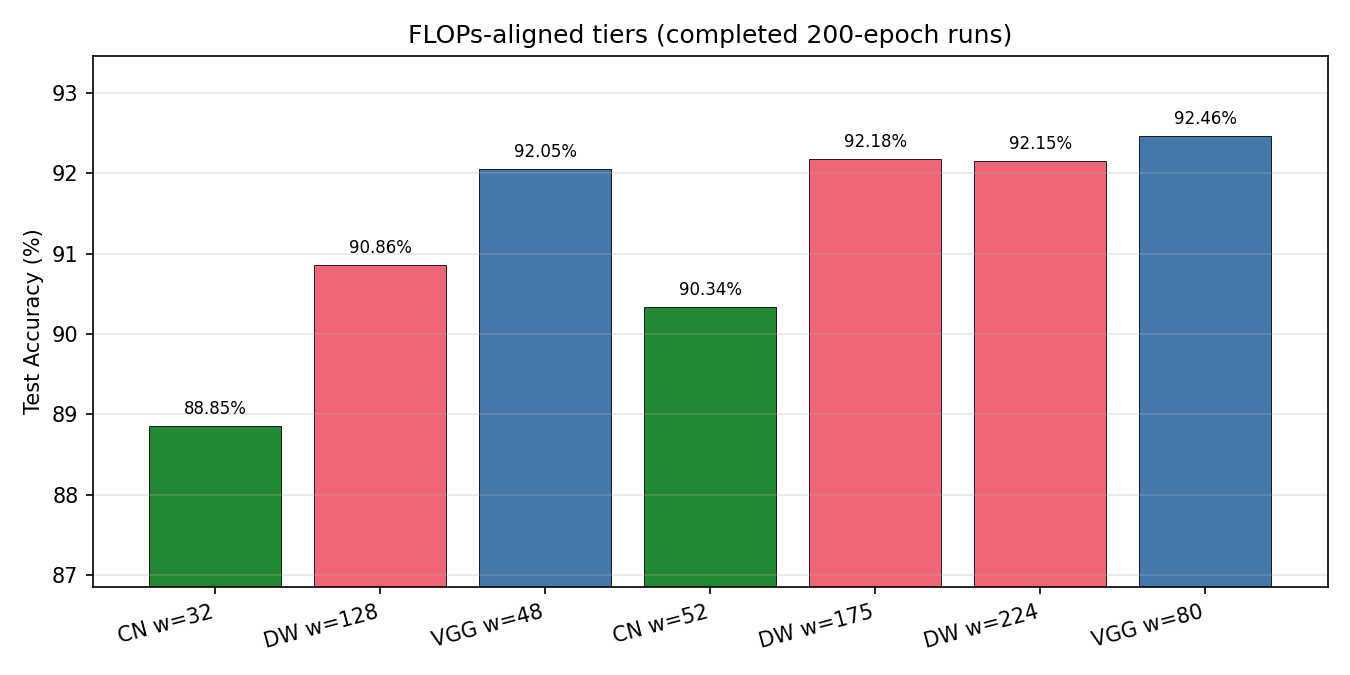
\includegraphics[width=\linewidth]{tier_test_accuracy.png}
    \caption{Per-tier test}
  \end{subfigure}\hfill
  \begin{subfigure}[t]{0.48\linewidth}
    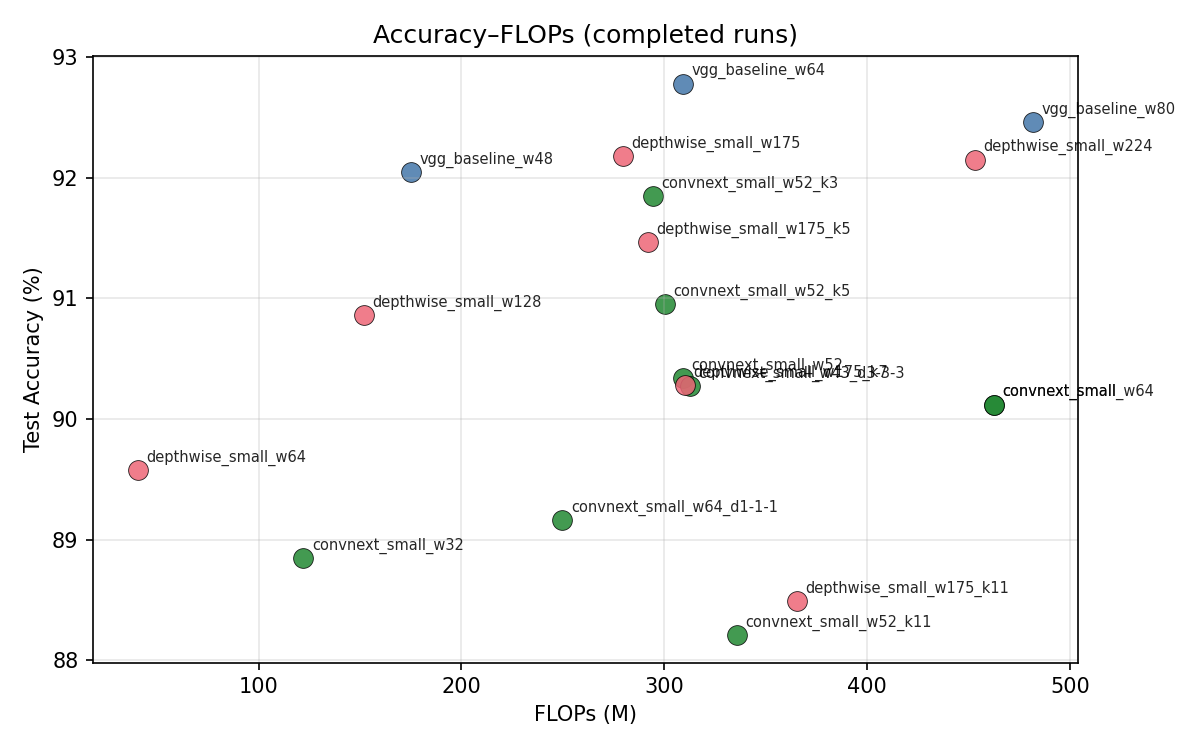
\includegraphics[width=\linewidth]{pareto_accuracy_flops.png}
    \caption{Pareto front}
  \end{subfigure}
  \caption{\grade{B/A} Tier comparison and accuracy--FLOPs Pareto.}
  \label{fig:main}
\end{figure}

\subsection{\grade{B/A} Width scaling (\grade{D/C})}

Fig.~\ref{fig:width}: within-family width increases FLOPs and usually test acc; cross-family, VGG leads in 175--310M. Table~\ref{tab:marginal}: VGG peaks at $w{=}64$; DW gains most low$\to$med (+1.04 pt/100M FLOPs); CN width helps but never catches VGG/DW.

\begin{table}[t]
  \caption{Marginal test gain (pt per 100M FLOPs).}
  \label{tab:marginal}
  \centering
  \scriptsize
  \begin{tabular}{@{}llrrr@{}}
    \toprule
    Family & Transition & $\Delta$FLOPs & $\Delta$test & Marginal \\
    \midrule
    VGG & $w{=}48{\to}64$ & +134M & +0.73 & +0.54 \\
    VGG & $w{=}64{\to}80$ & +172M & $-$0.32 & $-$0.19 \\
    DW & $w{=}128{\to}175$ & +127M & +1.32 & +1.04 \\
    DW & $w{=}175{\to}224$ & +174M & $-$0.03 & $-$0.02 \\
    CN & $w{=}32{\to}52$ & +187M & +1.49 & +0.80 \\
    CN & $w{=}52{\to}64$ & +153M & $-$0.22 & $-$0.14 \\
    \bottomrule
  \end{tabular}
\end{table}

\begin{figure}[t]
  \centering
  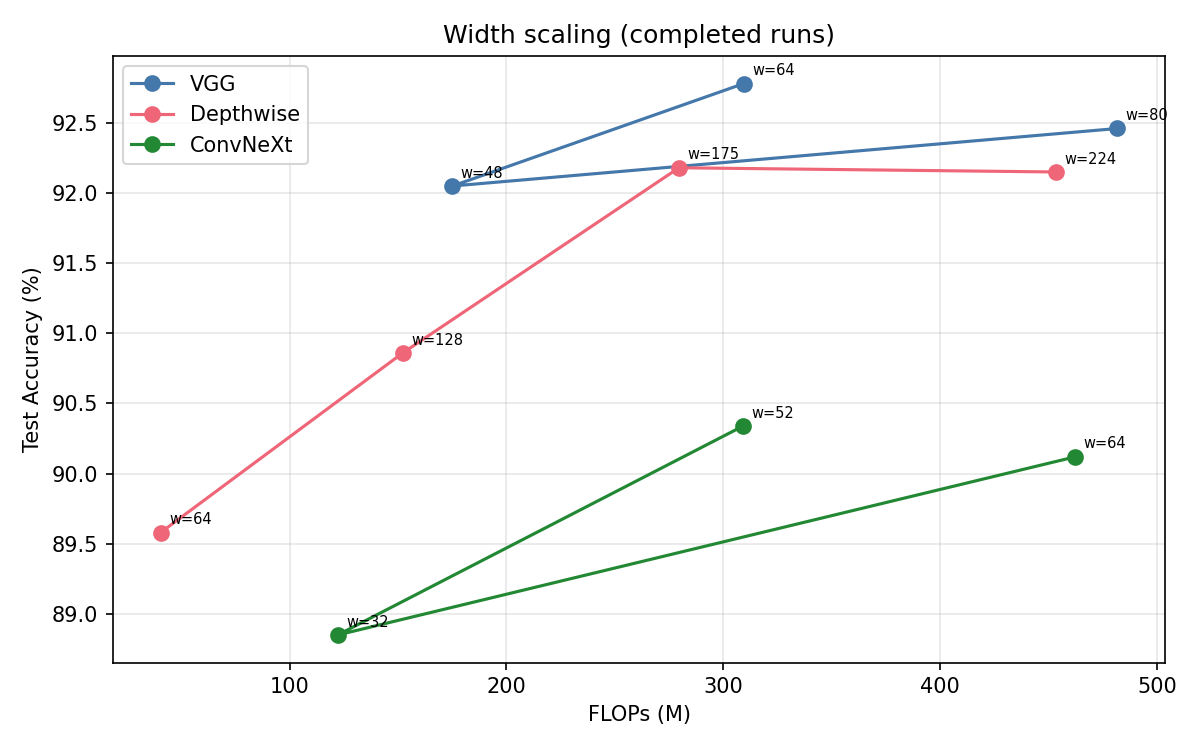
\includegraphics[width=0.68\linewidth]{width_scaling_accuracy_flops.png}
  \caption{Width scaling by family.}
  \label{fig:width}
\end{figure}

\subsection{\grade{B/A} Kernel ablation}

CN $w{=}52$, DW $w{=}175$; $k{\in}\{3,5,7,11\}$ (Table~\ref{tab:kernel}, Fig.~\ref{fig:kernel}). CN: 91.85$\to$90.95$\to$90.34$\to$88.21\%. DW: 92.18$\to$91.47$\to$90.28$\to$88.49\%; $k{=}11$ drops 3.69 pt vs.\ $k{=}3$. \textbf{RQ2 (kernel):} shrinking to $k{=}3$ is optimal; enlarging $k$ has \emph{negative} marginal return.

\begin{table}[t]
  \caption{Kernel scan (test \%). $^\dagger$: tier-default runs.}
  \label{tab:kernel}
  \centering
  \footnotesize
  \begin{tabular}{@{}crrrr@{}}
    \toprule
    $k$ & CN & DW & CN FLOPs & DW FLOPs \\
    \midrule
    3 & \textbf{91.85} & \textbf{92.18}$^\dagger$ & 294M & 280M$^\dagger$ \\
    5 & 90.95 & 91.47 & 300M & 292M \\
    7 & 90.34$^\dagger$ & 90.28 & 309M & 310M \\
    11 & 88.21 & 88.49 & 336M & 366M \\
    \bottomrule
  \end{tabular}
\end{table}

\begin{figure}[t]
  \centering
  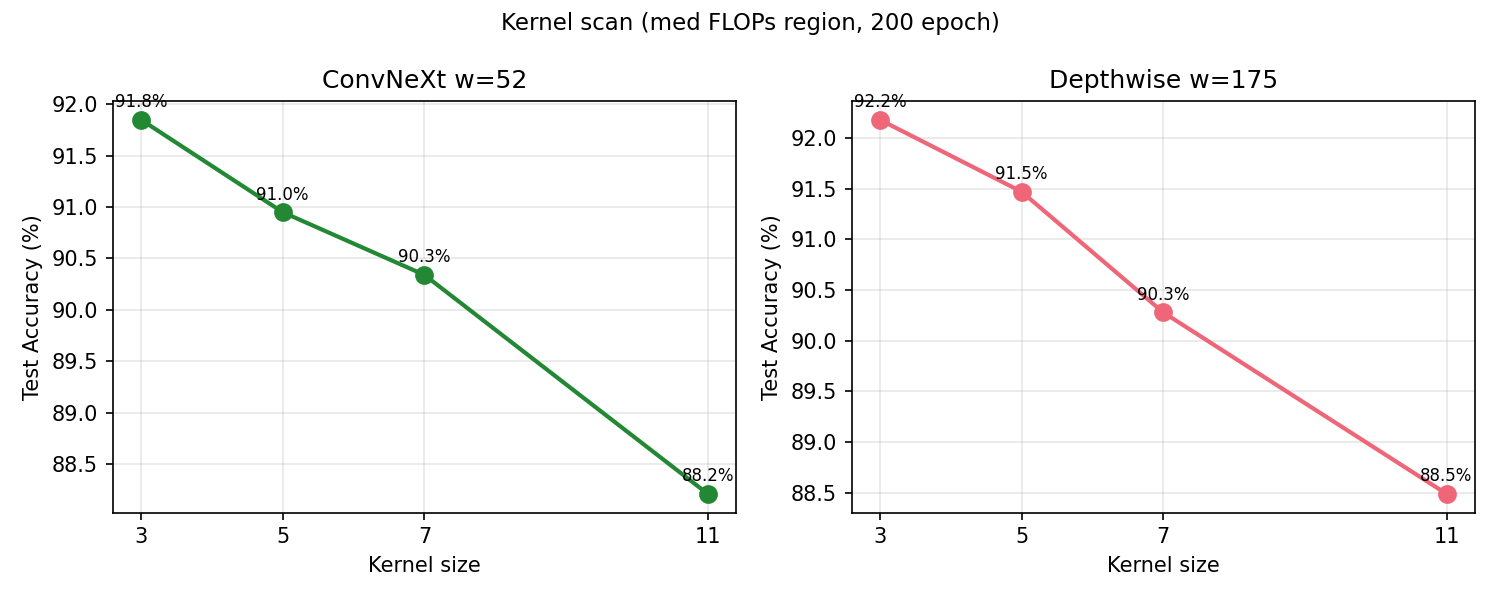
\includegraphics[width=0.55\linewidth]{kernel_scan_test_accuracy.png}
  \caption{Kernel scan.}
  \label{fig:kernel}
\end{figure}

\subsection{\grade{B/A} Depth and Pareto highlights}

Table~\ref{tab:depth}: shallow $(1,1,1)$ $w{=}64$ retrained to 89.16\% (was 41.67\% at 2 epochs); deep $(3,3,3)$ $w{=}43$ reaches 90.27\% but remains below VGG $w{=}48$ (92.05\% @ 175M). Table~\ref{tab:pareto}: non-dominated peak remains \texttt{vgg\_baseline\_w64}.

\begin{table}[t]
  \caption{ConvNeXt depth variants (200 epochs).}
  \label{tab:depth}
  \centering
  \footnotesize
  \begin{tabular}{@{}llrrrr@{}}
    \toprule
    depths & width & FLOPs & Val & Test & Note \\
    \midrule
    (2,2,2) & 64 & 462.4M & 91.40 & 90.12 & default \\
    (2,2,2) & 52 & 309.2M & 90.70 & 90.34 & med tier \\
    (1,1,1) & 64 & 249.8M & 90.90 & 89.16 & retrained \\
    (3,3,3) & 43 & 312.9M & 91.08 & 90.27 & deep \\
    \bottomrule
  \end{tabular}
\end{table}

\begin{table}[t]
  \caption{Selected Pareto points (by test accuracy).}
  \label{tab:pareto}
  \centering
  \scriptsize
  \begin{tabular}{@{}lrr@{}}
    \toprule
    run & FLOPs & Test \\
    \midrule
    vgg\_w64 & 309.5M & \textbf{92.78\%} \\
    vgg\_w48 & 175.1M & 92.05\% \\
    dw\_w175 & 279.6M & 92.18\% \\
    cn\_w52\_k3 & 294.3M & 91.85\% \\
    cn\_w52\_k11 & 336.1M & 88.21\% \\
    \bottomrule
  \end{tabular}
\end{table}

\begin{figure}[t]
  \centering
  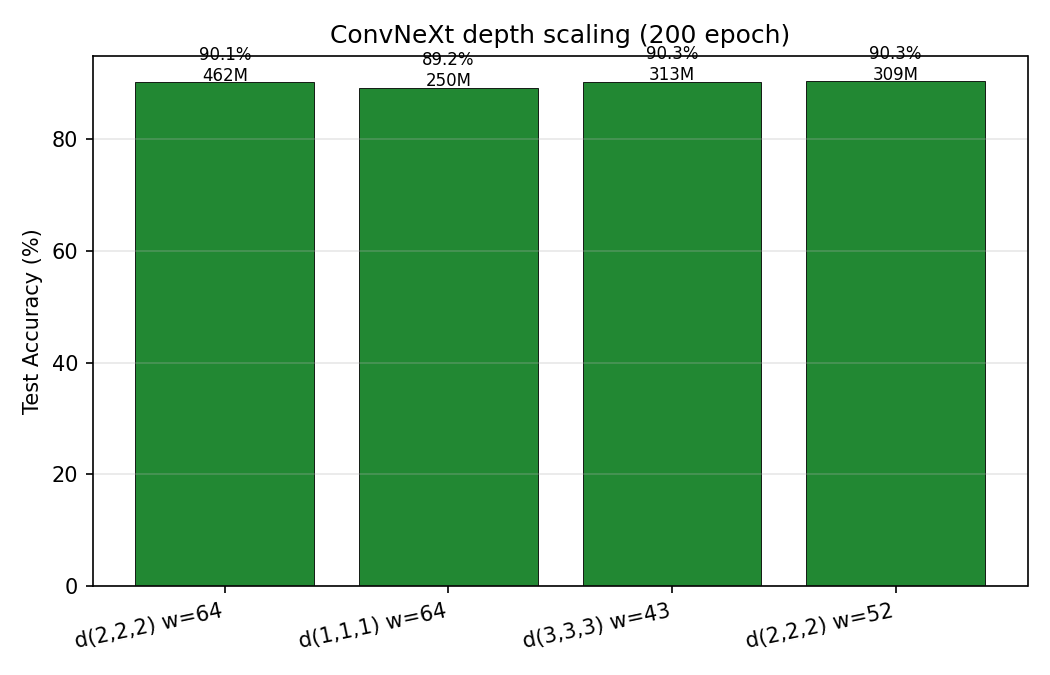
\includegraphics[width=0.55\linewidth]{depth_scan_test_accuracy.png}
  \caption{Depth variants vs.\ baselines.}
  \label{fig:depth}
\end{figure}

\section{Discussion and conclusions}
\label{sec:conc}

\subsection{Answers to RQ1 and RQ2}

\textbf{RQ1 (No).} Under matched FLOPs, ConvNeXt never beats VGG: gaps 3.20 pt (low), 2.44 pt (med), 2.34 pt (high). Best CN ($k{=}3$, 91.85\%) is still 0.93 pt below med-tier VGG. Modern blocks do \emph{not} improve the accuracy--FLOPs trade-off on CIFAR-10 under our recipe.

\textbf{RQ2.} Largest positive margins: \textbf{block type} (VGG $>$ DW $>$ CN) and \textbf{DW width} (low$\to$med). \textbf{Kernel enlargement} hurts both CN and DW. \textbf{Depth} only reorders CN variants.

\subsection{Architecture takeaway}

\begin{table}[t]
  \caption{Block families on CIFAR-10 (our sweep).}
  \label{tab:arch}
  \centering
  \footnotesize
  \begin{tabular}{@{}lccc@{}}
    \toprule
    Family & Accuracy & Efficiency & Recommendation \\
    \midrule
    VGG + BN & Highest & Medium & \textbf{Default choice} \\
    Depthwise & Near VGG & High & FLOPs-limited deploy \\
    ConvNeXt & Lower & Medium & Not recommended at $32{\times}32$ \\
    \bottomrule
  \end{tabular}
\end{table}

After three pools, feature maps are $\sim 4{\times}4$; $k{=}11$ likely over-smooths or adds boundary artifacts---ImageNet ConvNeXt priors do not transfer directly.

\subsection{Budget-aware rules and conclusion}

\begin{enumerate}[label=(\roman*)]
  \item Low FLOPs ($<{\sim}180$M): VGG $w{=}48$ (92.05\%); else DW $w{=}128$ (90.86\%).
  \item Med FLOPs ($\sim$280--330M): VGG $w{=}64$ (92.78\%); if FLOPs-limited, DW $w{=}175$ (92.18\%).
  \item High FLOPs: no gain vs.\ VGG $w{=}64$; avoid $w{=}80$.
  \item Kernels: use $k{=}3$; avoid $k{\geq}7$ on $32{\times}32$.
  \item CN depth: prefer $(2,2,2)$ or $(3,3,3)$ over $(1,1,1)$ unless FLOPs dominate.
\end{enumerate}

We completed 17/17 planned 200-epoch runs on a reproducible three-family benchmark. \textbf{VGG is Pareto-optimal}; \textbf{depthwise} is the best efficiency alternative; \textbf{ConvNeXt-style stacks} do not justify their compute when compared fairly.

\textbf{Limitations:} single seed; static FLOPs; no GPU latency/energy; MixUp/AMP off.

\begin{ack}
  DD2424 staff. Boyi Shi: model blocks; Puhao Zhu: FLOPs, Pareto, figures; Jinye Gong: pipeline and experiments.
\end{ack}

\bibliographystyle{plainnat}
\bibliography{references}

\end{document}
